


% Header, overrides base

    % Make sure that the sphinx doc style knows who it inherits from.
    \def\sphinxdocclass{article}

    % Declare the document class
    \documentclass[letterpaper,10pt,english]{/usr/share/sphinx/texinputs/sphinxhowto}

    % Imports
    \usepackage[utf8]{inputenc}
    \DeclareUnicodeCharacter{00A0}{\\nobreakspace}
    \usepackage[T1]{fontenc}
    \usepackage{babel}
    \usepackage{times}
    \usepackage{import}
    \usepackage[Bjarne]{/usr/share/sphinx/texinputs/fncychap}
    \usepackage{longtable}
    \usepackage{/usr/share/sphinx/texinputs/sphinx}
    \usepackage{multirow}

    \usepackage{amsmath}
    \usepackage{amssymb}
    \usepackage{ucs}
    \usepackage{enumerate}

    % Used to make the Input/Output rules follow around the contents.
    \usepackage{needspace}

    % Pygments requirements
    \usepackage{fancyvrb}
    \usepackage{color}
    % ansi colors additions
    \definecolor{darkgreen}{rgb}{.12,.54,.11}
    \definecolor{lightgray}{gray}{.95}
    \definecolor{brown}{rgb}{0.54,0.27,0.07}
    \definecolor{purple}{rgb}{0.5,0.0,0.5}
    \definecolor{darkgray}{gray}{0.25}
    \definecolor{lightred}{rgb}{1.0,0.39,0.28}
    \definecolor{lightgreen}{rgb}{0.48,0.99,0.0}
    \definecolor{lightblue}{rgb}{0.53,0.81,0.92}
    \definecolor{lightpurple}{rgb}{0.87,0.63,0.87}
    \definecolor{lightcyan}{rgb}{0.5,1.0,0.83}

    % Needed to box output/input
    \usepackage{tikz}
        \usetikzlibrary{calc,arrows,shadows}
    \usepackage[framemethod=tikz]{mdframed}

    \usepackage{alltt}

    % Used to load and display graphics
    \usepackage{graphicx}
    \graphicspath{ {figs/} }
    \usepackage[Export]{adjustbox} % To resize

    % used so that images for notebooks which have spaces in the name can still be included
    \usepackage{grffile}


    % For formatting output while also word wrapping.
    \usepackage{listings}
    \lstset{breaklines=true}
    \lstset{basicstyle=\small\ttfamily}
    \def\smaller{\fontsize{9.5pt}{9.5pt}\selectfont}

    %Pygments definitions
    
\makeatletter
\def\PY@reset{\let\PY@it=\relax \let\PY@bf=\relax%
    \let\PY@ul=\relax \let\PY@tc=\relax%
    \let\PY@bc=\relax \let\PY@ff=\relax}
\def\PY@tok#1{\csname PY@tok@#1\endcsname}
\def\PY@toks#1+{\ifx\relax#1\empty\else%
    \PY@tok{#1}\expandafter\PY@toks\fi}
\def\PY@do#1{\PY@bc{\PY@tc{\PY@ul{%
    \PY@it{\PY@bf{\PY@ff{#1}}}}}}}
\def\PY#1#2{\PY@reset\PY@toks#1+\relax+\PY@do{#2}}

\expandafter\def\csname PY@tok@gd\endcsname{\def\PY@tc##1{\textcolor[rgb]{0.63,0.00,0.00}{##1}}}
\expandafter\def\csname PY@tok@gu\endcsname{\let\PY@bf=\textbf\def\PY@tc##1{\textcolor[rgb]{0.50,0.00,0.50}{##1}}}
\expandafter\def\csname PY@tok@gt\endcsname{\def\PY@tc##1{\textcolor[rgb]{0.00,0.27,0.87}{##1}}}
\expandafter\def\csname PY@tok@gs\endcsname{\let\PY@bf=\textbf}
\expandafter\def\csname PY@tok@gr\endcsname{\def\PY@tc##1{\textcolor[rgb]{1.00,0.00,0.00}{##1}}}
\expandafter\def\csname PY@tok@cm\endcsname{\let\PY@it=\textit\def\PY@tc##1{\textcolor[rgb]{0.25,0.50,0.50}{##1}}}
\expandafter\def\csname PY@tok@vg\endcsname{\def\PY@tc##1{\textcolor[rgb]{0.10,0.09,0.49}{##1}}}
\expandafter\def\csname PY@tok@m\endcsname{\def\PY@tc##1{\textcolor[rgb]{0.40,0.40,0.40}{##1}}}
\expandafter\def\csname PY@tok@mh\endcsname{\def\PY@tc##1{\textcolor[rgb]{0.40,0.40,0.40}{##1}}}
\expandafter\def\csname PY@tok@go\endcsname{\def\PY@tc##1{\textcolor[rgb]{0.53,0.53,0.53}{##1}}}
\expandafter\def\csname PY@tok@ge\endcsname{\let\PY@it=\textit}
\expandafter\def\csname PY@tok@vc\endcsname{\def\PY@tc##1{\textcolor[rgb]{0.10,0.09,0.49}{##1}}}
\expandafter\def\csname PY@tok@il\endcsname{\def\PY@tc##1{\textcolor[rgb]{0.40,0.40,0.40}{##1}}}
\expandafter\def\csname PY@tok@cs\endcsname{\let\PY@it=\textit\def\PY@tc##1{\textcolor[rgb]{0.25,0.50,0.50}{##1}}}
\expandafter\def\csname PY@tok@cp\endcsname{\def\PY@tc##1{\textcolor[rgb]{0.74,0.48,0.00}{##1}}}
\expandafter\def\csname PY@tok@gi\endcsname{\def\PY@tc##1{\textcolor[rgb]{0.00,0.63,0.00}{##1}}}
\expandafter\def\csname PY@tok@gh\endcsname{\let\PY@bf=\textbf\def\PY@tc##1{\textcolor[rgb]{0.00,0.00,0.50}{##1}}}
\expandafter\def\csname PY@tok@ni\endcsname{\let\PY@bf=\textbf\def\PY@tc##1{\textcolor[rgb]{0.60,0.60,0.60}{##1}}}
\expandafter\def\csname PY@tok@nl\endcsname{\def\PY@tc##1{\textcolor[rgb]{0.63,0.63,0.00}{##1}}}
\expandafter\def\csname PY@tok@nn\endcsname{\let\PY@bf=\textbf\def\PY@tc##1{\textcolor[rgb]{0.00,0.00,1.00}{##1}}}
\expandafter\def\csname PY@tok@no\endcsname{\def\PY@tc##1{\textcolor[rgb]{0.53,0.00,0.00}{##1}}}
\expandafter\def\csname PY@tok@na\endcsname{\def\PY@tc##1{\textcolor[rgb]{0.49,0.56,0.16}{##1}}}
\expandafter\def\csname PY@tok@nb\endcsname{\def\PY@tc##1{\textcolor[rgb]{0.00,0.50,0.00}{##1}}}
\expandafter\def\csname PY@tok@nc\endcsname{\let\PY@bf=\textbf\def\PY@tc##1{\textcolor[rgb]{0.00,0.00,1.00}{##1}}}
\expandafter\def\csname PY@tok@nd\endcsname{\def\PY@tc##1{\textcolor[rgb]{0.67,0.13,1.00}{##1}}}
\expandafter\def\csname PY@tok@ne\endcsname{\let\PY@bf=\textbf\def\PY@tc##1{\textcolor[rgb]{0.82,0.25,0.23}{##1}}}
\expandafter\def\csname PY@tok@nf\endcsname{\def\PY@tc##1{\textcolor[rgb]{0.00,0.00,1.00}{##1}}}
\expandafter\def\csname PY@tok@si\endcsname{\let\PY@bf=\textbf\def\PY@tc##1{\textcolor[rgb]{0.73,0.40,0.53}{##1}}}
\expandafter\def\csname PY@tok@s2\endcsname{\def\PY@tc##1{\textcolor[rgb]{0.73,0.13,0.13}{##1}}}
\expandafter\def\csname PY@tok@vi\endcsname{\def\PY@tc##1{\textcolor[rgb]{0.10,0.09,0.49}{##1}}}
\expandafter\def\csname PY@tok@nt\endcsname{\let\PY@bf=\textbf\def\PY@tc##1{\textcolor[rgb]{0.00,0.50,0.00}{##1}}}
\expandafter\def\csname PY@tok@nv\endcsname{\def\PY@tc##1{\textcolor[rgb]{0.10,0.09,0.49}{##1}}}
\expandafter\def\csname PY@tok@s1\endcsname{\def\PY@tc##1{\textcolor[rgb]{0.73,0.13,0.13}{##1}}}
\expandafter\def\csname PY@tok@sh\endcsname{\def\PY@tc##1{\textcolor[rgb]{0.73,0.13,0.13}{##1}}}
\expandafter\def\csname PY@tok@sc\endcsname{\def\PY@tc##1{\textcolor[rgb]{0.73,0.13,0.13}{##1}}}
\expandafter\def\csname PY@tok@sx\endcsname{\def\PY@tc##1{\textcolor[rgb]{0.00,0.50,0.00}{##1}}}
\expandafter\def\csname PY@tok@bp\endcsname{\def\PY@tc##1{\textcolor[rgb]{0.00,0.50,0.00}{##1}}}
\expandafter\def\csname PY@tok@c1\endcsname{\let\PY@it=\textit\def\PY@tc##1{\textcolor[rgb]{0.25,0.50,0.50}{##1}}}
\expandafter\def\csname PY@tok@kc\endcsname{\let\PY@bf=\textbf\def\PY@tc##1{\textcolor[rgb]{0.00,0.50,0.00}{##1}}}
\expandafter\def\csname PY@tok@c\endcsname{\let\PY@it=\textit\def\PY@tc##1{\textcolor[rgb]{0.25,0.50,0.50}{##1}}}
\expandafter\def\csname PY@tok@mf\endcsname{\def\PY@tc##1{\textcolor[rgb]{0.40,0.40,0.40}{##1}}}
\expandafter\def\csname PY@tok@err\endcsname{\def\PY@bc##1{\setlength{\fboxsep}{0pt}\fcolorbox[rgb]{1.00,0.00,0.00}{1,1,1}{\strut ##1}}}
\expandafter\def\csname PY@tok@kd\endcsname{\let\PY@bf=\textbf\def\PY@tc##1{\textcolor[rgb]{0.00,0.50,0.00}{##1}}}
\expandafter\def\csname PY@tok@ss\endcsname{\def\PY@tc##1{\textcolor[rgb]{0.10,0.09,0.49}{##1}}}
\expandafter\def\csname PY@tok@sr\endcsname{\def\PY@tc##1{\textcolor[rgb]{0.73,0.40,0.53}{##1}}}
\expandafter\def\csname PY@tok@mo\endcsname{\def\PY@tc##1{\textcolor[rgb]{0.40,0.40,0.40}{##1}}}
\expandafter\def\csname PY@tok@kn\endcsname{\let\PY@bf=\textbf\def\PY@tc##1{\textcolor[rgb]{0.00,0.50,0.00}{##1}}}
\expandafter\def\csname PY@tok@mi\endcsname{\def\PY@tc##1{\textcolor[rgb]{0.40,0.40,0.40}{##1}}}
\expandafter\def\csname PY@tok@gp\endcsname{\let\PY@bf=\textbf\def\PY@tc##1{\textcolor[rgb]{0.00,0.00,0.50}{##1}}}
\expandafter\def\csname PY@tok@o\endcsname{\def\PY@tc##1{\textcolor[rgb]{0.40,0.40,0.40}{##1}}}
\expandafter\def\csname PY@tok@kr\endcsname{\let\PY@bf=\textbf\def\PY@tc##1{\textcolor[rgb]{0.00,0.50,0.00}{##1}}}
\expandafter\def\csname PY@tok@s\endcsname{\def\PY@tc##1{\textcolor[rgb]{0.73,0.13,0.13}{##1}}}
\expandafter\def\csname PY@tok@kp\endcsname{\def\PY@tc##1{\textcolor[rgb]{0.00,0.50,0.00}{##1}}}
\expandafter\def\csname PY@tok@w\endcsname{\def\PY@tc##1{\textcolor[rgb]{0.73,0.73,0.73}{##1}}}
\expandafter\def\csname PY@tok@kt\endcsname{\def\PY@tc##1{\textcolor[rgb]{0.69,0.00,0.25}{##1}}}
\expandafter\def\csname PY@tok@ow\endcsname{\let\PY@bf=\textbf\def\PY@tc##1{\textcolor[rgb]{0.67,0.13,1.00}{##1}}}
\expandafter\def\csname PY@tok@sb\endcsname{\def\PY@tc##1{\textcolor[rgb]{0.73,0.13,0.13}{##1}}}
\expandafter\def\csname PY@tok@k\endcsname{\let\PY@bf=\textbf\def\PY@tc##1{\textcolor[rgb]{0.00,0.50,0.00}{##1}}}
\expandafter\def\csname PY@tok@se\endcsname{\let\PY@bf=\textbf\def\PY@tc##1{\textcolor[rgb]{0.73,0.40,0.13}{##1}}}
\expandafter\def\csname PY@tok@sd\endcsname{\let\PY@it=\textit\def\PY@tc##1{\textcolor[rgb]{0.73,0.13,0.13}{##1}}}

\def\PYZbs{\char`\\}
\def\PYZus{\char`\_}
\def\PYZob{\char`\{}
\def\PYZcb{\char`\}}
\def\PYZca{\char`\^}
\def\PYZam{\char`\&}
\def\PYZlt{\char`\<}
\def\PYZgt{\char`\>}
\def\PYZsh{\char`\#}
\def\PYZpc{\char`\%}
\def\PYZdl{\char`\$}
\def\PYZhy{\char`\-}
\def\PYZsq{\char`\'}
\def\PYZdq{\char`\"}
\def\PYZti{\char`\~}
% for compatibility with earlier versions
\def\PYZat{@}
\def\PYZlb{[}
\def\PYZrb{]}
\makeatother


    %Set pygments styles if needed...
    
        \definecolor{nbframe-border}{rgb}{0.867,0.867,0.867}
        \definecolor{nbframe-bg}{rgb}{0.969,0.969,0.969}
        \definecolor{nbframe-in-prompt}{rgb}{0.0,0.0,0.502}
        \definecolor{nbframe-out-prompt}{rgb}{0.545,0.0,0.0}

        \newenvironment{ColorVerbatim}
        {\begin{mdframed}[%
            roundcorner=1.0pt, %
            backgroundcolor=nbframe-bg, %
            userdefinedwidth=1\linewidth, %
            leftmargin=0.1\linewidth, %
            innerleftmargin=0pt, %
            innerrightmargin=0pt, %
            linecolor=nbframe-border, %
            linewidth=1pt, %
            usetwoside=false, %
            everyline=true, %
            innerlinewidth=3pt, %
            innerlinecolor=nbframe-bg, %
            middlelinewidth=1pt, %
            middlelinecolor=nbframe-bg, %
            outerlinewidth=0.5pt, %
            outerlinecolor=nbframe-border, %
            needspace=0pt
        ]}
        {\end{mdframed}}
        
        \newenvironment{InvisibleVerbatim}
        {\begin{mdframed}[leftmargin=0.1\linewidth,innerleftmargin=3pt,innerrightmargin=3pt, userdefinedwidth=1\linewidth, linewidth=0pt, linecolor=white, usetwoside=false]}
        {\end{mdframed}}

        \renewenvironment{Verbatim}[1][\unskip]
        {\begin{alltt}\smaller}
        {\end{alltt}}
    

    % Help prevent overflowing lines due to urls and other hard-to-break 
    % entities.  This doesn't catch everything...
    \sloppy

    % Document level variables
    \title{pandas\_toGo-slides}
    \date{March 25, 2015}
    \release{}
%     \author{Unknown Author}
    \renewcommand{\releasename}{}

    % TODO: Add option for the user to specify a logo for his/her export.
    \newcommand{\sphinxlogo}{}

    % Make the index page of the document.
    \makeindex

    % Import sphinx document type specifics.
     


% Body

    % Start of the document
    \begin{document}

        
            \maketitle
        

        


        
        
Pandas tutorial for the Master in Neurosciences.

Florencia Noriega
July 2014

% Start slideshow with: ipython nbconvert
% pandas\_tutorial\_Sose2014-slides.ipynb --to slides --post serve
% create pdf:
% ipython nbconvert pandas\_toGo-slides.ipynb --to latex


    % Make sure that atleast 4 lines are below the HR
    \needspace{4\baselineskip}

    
        \vspace{6pt}
        \makebox[0.1\linewidth]{\smaller\hfill\tt\color{nbframe-in-prompt}In\hspace{4pt}{[}55{]}:\hspace{4pt}}\\*
        \vspace{-2.65\baselineskip}
        \begin{ColorVerbatim}
            \vspace{-0.7\baselineskip}
            \begin{Verbatim}[commandchars=\\\{\}]
\PY{k+kn}{import} \PY{n+nn}{pandas} \PY{k+kn}{as} \PY{n+nn}{pd}
\PY{k+kn}{import} \PY{n+nn}{matplotlib.pyplot} \PY{k+kn}{as} \PY{n+nn}{plt}
\PY{k+kn}{import} \PY{n+nn}{numpy} \PY{k+kn}{as} \PY{n+nn}{np}
\PY{k+kn}{from} \PY{n+nn}{IPython.display} \PY{k+kn}{import} \PY{n}{Image} \PY{c}{\PYZsh{} for the showing of images}

\PY{c}{\PYZsh{}http://en.wikipedia.org/wiki/Subtropics\PYZsh{}mediaviewer/File:World\PYZus{}map\PYZus{}indicating\PYZus{}tropics\PYZus{}and\PYZus{}subtropics.png}
\PY{c}{\PYZsh{}pandas = Image(\PYZsq{}./panditaBambu.jpg\PYZsq{}, width=(100,100)) }
\PY{n}{bye} \PY{o}{=} \PY{n}{Image}\PY{p}{(}\PY{l+s}{\PYZsq{}}\PY{l+s}{./images/panditaBye.png}\PY{l+s}{\PYZsq{}}\PY{p}{,} \PY{n}{width}\PY{o}{=}\PY{p}{(}\PY{l+m+mi}{100}\PY{p}{,}\PY{l+m+mi}{100}\PY{p}{)}\PY{p}{)} 
\PY{c}{\PYZsh{}longitude = Image(\PYZsq{}./longitude.png\PYZsq{}, width=(100,100)) \PYZsh{} wikipedia}

\PY{o}{\PYZpc{}}\PY{k}{matplotlib} \PY{n}{inline}
\end{Verbatim}

            
                \vspace{-0.2\baselineskip}
            
        \end{ColorVerbatim}
    
\part{Pandas}\textbf{References:}

\begin{itemize}
\itemsep1pt\parskip0pt\parsep0pt
\item
  http://pandas.pydata.org/
\item
  Cookbook --- pandas 0.14.0 documentation
\end{itemize}\section{Reading CSV files}

    % Make sure that atleast 4 lines are below the HR
    \needspace{4\baselineskip}

    
        \vspace{6pt}
        \makebox[0.1\linewidth]{\smaller\hfill\tt\color{nbframe-in-prompt}In\hspace{4pt}{[}21{]}:\hspace{4pt}}\\*
        \vspace{-2.65\baselineskip}
        \begin{ColorVerbatim}
            \vspace{-0.7\baselineskip}
            \begin{Verbatim}[commandchars=\\\{\}]
\PY{n}{D} \PY{o}{=} \PY{n}{pd}\PY{o}{.}\PY{n}{read\PYZus{}csv}\PY{p}{(}\PY{l+s}{\PYZdq{}}\PY{l+s}{amazonianBirds.csv}\PY{l+s}{\PYZdq{}}\PY{p}{)}\PY{c}{\PYZsh{}, sep = \PYZsq{},\PYZsq{}) \PYZsh{} data obtaied from http://www.xeno\PYZhy{}canto.org/}
\end{Verbatim}

            
                \vspace{-0.2\baselineskip}
            
        \end{ColorVerbatim}
    
\section{What is in this csv file?}Number of lines, names of the columns?

    % Make sure that atleast 4 lines are below the HR
    \needspace{4\baselineskip}

    
        \vspace{6pt}
        \makebox[0.1\linewidth]{\smaller\hfill\tt\color{nbframe-in-prompt}In\hspace{4pt}{[}22{]}:\hspace{4pt}}\\*
        \vspace{-2.65\baselineskip}
        \begin{ColorVerbatim}
            \vspace{-0.7\baselineskip}
            \begin{Verbatim}[commandchars=\\\{\}]
\PY{n}{colNames} \PY{o}{=} \PY{n}{D}\PY{o}{.}\PY{n}{columns}\PY{o}{.}\PY{n}{values} \PY{c}{\PYZsh{} names of the columns}
\PY{k}{print} \PY{l+s}{\PYZdq{}}\PY{l+s}{* length of the file:}\PY{l+s}{\PYZdq{}}\PY{p}{,} \PY{n+nb}{len}\PY{p}{(}\PY{n}{D}\PY{p}{)}\PY{p}{,} \PY{l+s}{\PYZdq{}}\PY{l+s+se}{\PYZbs{}n}\PY{l+s}{* names of the columns (}\PY{l+s+si}{\PYZpc{}d}\PY{l+s}{):}\PY{l+s+se}{\PYZbs{}n}\PY{l+s}{\PYZdq{}}\PY{o}{\PYZpc{}}\PY{k}{len}\PY{p}{(}\PY{n}{colNames}\PY{p}{)}\PY{p}{,} \PY{n}{colNames}
\end{Verbatim}

            
                \vspace{-0.2\baselineskip}
            
        \end{ColorVerbatim}
    

    

        % If the first block is an image, minipage the image.  Else
        % request a certain amount of space for the input text.
        \needspace{4\baselineskip}
        
        

            % Add document contents.
            
                \begin{InvisibleVerbatim}
                \vspace{-0.5\baselineskip}
\begin{alltt}* length of the file: 8588
* names of the columns (7):
['recordist' 'date' 'time' 'location' 'longitude' 'latitude'
'elevation']
\end{alltt}

            \end{InvisibleVerbatim}
            
        
    
Get a taste of the file

    % Make sure that atleast 4 lines are below the HR
    \needspace{4\baselineskip}

    
        \vspace{6pt}
        \makebox[0.1\linewidth]{\smaller\hfill\tt\color{nbframe-in-prompt}In\hspace{4pt}{[}23{]}:\hspace{4pt}}\\*
        \vspace{-2.65\baselineskip}
        \begin{ColorVerbatim}
            \vspace{-0.7\baselineskip}
            \begin{Verbatim}[commandchars=\\\{\}]
\PY{n}{D}\PY{o}{.}\PY{n}{head}\PY{p}{(}\PY{p}{)} \PY{c}{\PYZsh{} shows the first 5 lines, try D.tail()}
\end{Verbatim}

            
                \vspace{-0.2\baselineskip}
            
        \end{ColorVerbatim}
    

    

        % If the first block is an image, minipage the image.  Else
        % request a certain amount of space for the input text.
        \needspace{4\baselineskip}
        
        

            % Add document contents.
            
                \makebox[0.1\linewidth]{\smaller\hfill\tt\color{nbframe-out-prompt}Out\hspace{4pt}{[}23{]}:\hspace{4pt}}\\*
                \vspace{-2.55\baselineskip}\begin{InvisibleVerbatim}
                \vspace{-0.5\baselineskip}
\begin{alltt}      recordist        date   time  \textbackslash{}
0   Daniel Lane  2011-02-24  05:55
1   Daniel Lane  2011-02-24  06:05
2  Eric DeFonso  2011-09-03  18:00
3  Eric DeFonso  2011-09-04  06:00
4  Eric DeFonso  2011-09-04  06:05

                                         location  longitude  latitude
\textbackslash{}
0  10 km S Pocone on Transpantaneira, Mato Grosso   -56.6480  -16.3620
1  10 km S Pocone on Transpantaneira, Mato Grosso   -56.6480  -16.3620
2                    Pantanal Wildlife Center, MT   -56.8764  -16.7581
3                    Pantanal Wildlife Center, MT   -56.8764  -16.7581
4                    Pantanal Wildlife Center, MT   -56.8764  -16.7581

  elevation
0       115
1       115
2       110
3       110
4       110

[5 rows x 7 columns]\end{alltt}

            \end{InvisibleVerbatim}
            
        
    
\part{Selecting and plotting a column}\subsection{Selecting a column from the data frame}

    % Make sure that atleast 4 lines are below the HR
    \needspace{4\baselineskip}

    
        \vspace{6pt}
        \makebox[0.1\linewidth]{\smaller\hfill\tt\color{nbframe-in-prompt}In\hspace{4pt}{[}24{]}:\hspace{4pt}}\\*
        \vspace{-2.65\baselineskip}
        \begin{ColorVerbatim}
            \vspace{-0.7\baselineskip}
            \begin{Verbatim}[commandchars=\\\{\}]
\PY{k}{print} \PY{n+nb}{len}\PY{p}{(}\PY{n}{D}\PY{o}{.}\PY{n}{longitude}\PY{p}{)}
\PY{n}{D}\PY{o}{.}\PY{n}{longitude}\PY{p}{[}\PY{p}{:}\PY{l+m+mi}{3}\PY{p}{]}
\end{Verbatim}

            
                \vspace{-0.2\baselineskip}
            
        \end{ColorVerbatim}
    

    

        % If the first block is an image, minipage the image.  Else
        % request a certain amount of space for the input text.
        \needspace{4\baselineskip}
        
        

            % Add document contents.
            
                \begin{InvisibleVerbatim}
                \vspace{-0.5\baselineskip}
\begin{alltt}8588
\end{alltt}

            \end{InvisibleVerbatim}
            
                \makebox[0.1\linewidth]{\smaller\hfill\tt\color{nbframe-out-prompt}Out\hspace{4pt}{[}24{]}:\hspace{4pt}}\\*
                \vspace{-2.55\baselineskip}\begin{InvisibleVerbatim}
                \vspace{-0.5\baselineskip}
\begin{alltt}0   -56.6480
1   -56.6480
2   -56.8764
Name: longitude, dtype: float64\end{alltt}

            \end{InvisibleVerbatim}
            
        
    
\section{Plotting the data}\subsection{Plotting a column}

    % Make sure that atleast 4 lines are below the HR
    \needspace{4\baselineskip}

    
        \vspace{6pt}
        \makebox[0.1\linewidth]{\smaller\hfill\tt\color{nbframe-in-prompt}In\hspace{4pt}{[}25{]}:\hspace{4pt}}\\*
        \vspace{-2.65\baselineskip}
        \begin{ColorVerbatim}
            \vspace{-0.7\baselineskip}
            \begin{Verbatim}[commandchars=\\\{\}]
\PY{n}{D}\PY{p}{[}\PY{l+s}{\PYZsq{}}\PY{l+s}{longitude}\PY{l+s}{\PYZsq{}}\PY{p}{]}\PY{o}{.}\PY{n}{plot}\PY{p}{(} \PY{n}{title} \PY{o}{=} \PY{l+s}{\PYZsq{}}\PY{l+s}{Longitude}\PY{l+s}{\PYZsq{}}\PY{p}{)}
\PY{n}{D}\PY{p}{[}\PY{l+s}{\PYZsq{}}\PY{l+s}{latitude}\PY{l+s}{\PYZsq{}}\PY{p}{]}\PY{o}{.}\PY{n}{plot}\PY{p}{(} \PY{n}{title} \PY{o}{=} \PY{l+s}{\PYZsq{}}\PY{l+s}{latitude}\PY{l+s}{\PYZsq{}}\PY{p}{)}
\PY{n}{plt}\PY{o}{.}\PY{n}{savefig}\PY{p}{(}\PY{l+s}{\PYZsq{}}\PY{l+s}{images/series.png}\PY{l+s}{\PYZsq{}}\PY{p}{)}
\end{Verbatim}

            
                \vspace{-0.2\baselineskip}
            
        \end{ColorVerbatim}
    

    

        % If the first block is an image, minipage the image.  Else
        % request a certain amount of space for the input text.
        \needspace{4\baselineskip}
        
        

            % Add document contents.
            
                \begin{InvisibleVerbatim}
                \vspace{-0.5\baselineskip}
    \begin{center}
    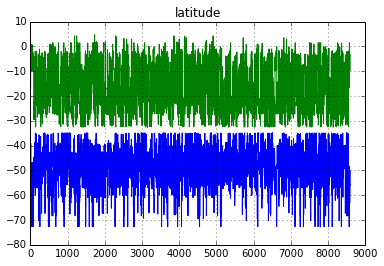
\includegraphics[max size={\textwidth}{\textheight}]{pandas_toGo-slides_files/pandas_toGo-slides_17_0.png}
    \par
    \end{center}
    
            \end{InvisibleVerbatim}
            
        
    
\subsection{Scatter plot with two columns}

    % Make sure that atleast 4 lines are below the HR
    \needspace{4\baselineskip}

    
        \vspace{6pt}
        \makebox[0.1\linewidth]{\smaller\hfill\tt\color{nbframe-in-prompt}In\hspace{4pt}{[}26{]}:\hspace{4pt}}\\*
        \vspace{-2.65\baselineskip}
        \begin{ColorVerbatim}
            \vspace{-0.7\baselineskip}
            \begin{Verbatim}[commandchars=\\\{\}]
\PY{n}{plt}\PY{o}{.}\PY{n}{scatter}\PY{p}{(}\PY{n}{D}\PY{o}{.}\PY{n}{longitude}\PY{p}{,} \PY{n}{D}\PY{o}{.}\PY{n}{latitude}\PY{p}{)}
\PY{n}{plt}\PY{o}{.}\PY{n}{xlabel}\PY{p}{(}\PY{l+s}{\PYZsq{}}\PY{l+s}{longitude}\PY{l+s}{\PYZsq{}}\PY{p}{)}
\PY{n}{plt}\PY{o}{.}\PY{n}{ylabel}\PY{p}{(}\PY{l+s}{\PYZsq{}}\PY{l+s}{latitude}\PY{l+s}{\PYZsq{}}\PY{p}{)}
\PY{n}{plt}\PY{o}{.}\PY{n}{xlim}\PY{p}{(}\PY{o}{\PYZhy{}}\PY{l+m+mi}{100}\PY{p}{,} \PY{o}{\PYZhy{}}\PY{l+m+mi}{20}\PY{p}{)}

\PY{n}{plt}\PY{o}{.}\PY{n}{savefig}\PY{p}{(}\PY{l+s}{\PYZdq{}}\PY{l+s}{scattpl.png}\PY{l+s}{\PYZdq{}}\PY{p}{)}
\end{Verbatim}

            
                \vspace{-0.2\baselineskip}
            
        \end{ColorVerbatim}
    

    

        % If the first block is an image, minipage the image.  Else
        % request a certain amount of space for the input text.
        \needspace{4\baselineskip}
        
        

            % Add document contents.
            
                \begin{InvisibleVerbatim}
                \vspace{-0.5\baselineskip}
    \begin{center}
    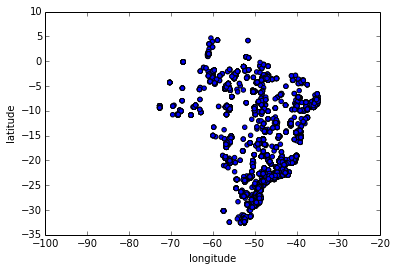
\includegraphics[max size={\textwidth}{\textheight}]{pandas_toGo-slides_files/pandas_toGo-slides_19_0.png}
    \par
    \end{center}
    
            \end{InvisibleVerbatim}
            
        
    
\subsection{Plotting histograms}

    % Make sure that atleast 4 lines are below the HR
    \needspace{4\baselineskip}

    
        \vspace{6pt}
        \makebox[0.1\linewidth]{\smaller\hfill\tt\color{nbframe-in-prompt}In\hspace{4pt}{[}27{]}:\hspace{4pt}}\\*
        \vspace{-2.65\baselineskip}
        \begin{ColorVerbatim}
            \vspace{-0.7\baselineskip}
            \begin{Verbatim}[commandchars=\\\{\}]
\PY{n}{x1} \PY{o}{=} \PY{l+s}{\PYZsq{}}\PY{l+s}{longitude}\PY{l+s}{\PYZsq{}}
\PY{n}{x2} \PY{o}{=} \PY{l+s}{\PYZsq{}}\PY{l+s}{latitude}\PY{l+s}{\PYZsq{}}
\PY{n}{plt}\PY{o}{.}\PY{n}{hist}\PY{p}{(}\PY{n}{D}\PY{p}{[}\PY{n}{x1}\PY{p}{]}\PY{p}{,} \PY{n}{label} \PY{o}{=} \PY{n}{x1}\PY{p}{)}
\PY{n}{plt}\PY{o}{.}\PY{n}{hist}\PY{p}{(}\PY{n}{D}\PY{p}{[}\PY{n}{x2}\PY{p}{]}\PY{p}{,} \PY{n}{label} \PY{o}{=} \PY{n}{x2}\PY{p}{)}
\PY{n}{plt}\PY{o}{.}\PY{n}{legend}\PY{p}{(}\PY{p}{)}

\PY{n}{plt}\PY{o}{.}\PY{n}{savefig}\PY{p}{(}\PY{l+s}{\PYZdq{}}\PY{l+s}{histp.png}\PY{l+s}{\PYZdq{}}\PY{p}{)}
\end{Verbatim}

            
                \vspace{-0.2\baselineskip}
            
        \end{ColorVerbatim}
    

    

        % If the first block is an image, minipage the image.  Else
        % request a certain amount of space for the input text.
        \needspace{4\baselineskip}
        
        

            % Add document contents.
            
                \begin{InvisibleVerbatim}
                \vspace{-0.5\baselineskip}
    \begin{center}
    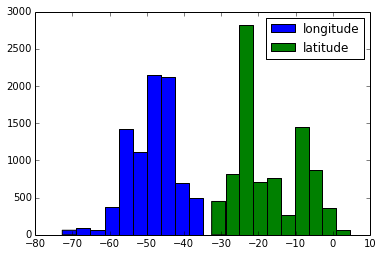
\includegraphics[max size={\textwidth}{\textheight}]{pandas_toGo-slides_files/pandas_toGo-slides_21_0.png}
    \par
    \end{center}
    
            \end{InvisibleVerbatim}
            
        
    
\part{Selecting data}\subsubsection{Symmetry}

    % Make sure that atleast 4 lines are below the HR
    \needspace{4\baselineskip}

    
        \vspace{6pt}
        \makebox[0.1\linewidth]{\smaller\hfill\tt\color{nbframe-in-prompt}In\hspace{4pt}{[}28{]}:\hspace{4pt}}\\*
        \vspace{-2.65\baselineskip}
        \begin{ColorVerbatim}
            \vspace{-0.7\baselineskip}
            \begin{Verbatim}[commandchars=\\\{\}]
\PY{n}{D}\PY{p}{[}\PY{l+s}{\PYZsq{}}\PY{l+s}{date}\PY{l+s}{\PYZsq{}}\PY{p}{]}\PY{p}{[}\PY{p}{:}\PY{l+m+mi}{5}\PY{p}{]} \PY{c}{\PYZsh{} first five elements}
\PY{n}{D}\PY{p}{[}\PY{p}{:}\PY{l+m+mi}{5}\PY{p}{]}\PY{p}{[}\PY{l+s}{\PYZsq{}}\PY{l+s}{date}\PY{l+s}{\PYZsq{}}\PY{p}{]}
\PY{n}{D}\PY{o}{.}\PY{n}{date}\PY{p}{[}\PY{p}{:}\PY{l+m+mi}{5}\PY{p}{]}
\end{Verbatim}

            
                \vspace{-0.2\baselineskip}
            
        \end{ColorVerbatim}
    

    

        % If the first block is an image, minipage the image.  Else
        % request a certain amount of space for the input text.
        \needspace{4\baselineskip}
        
        

            % Add document contents.
            
                \makebox[0.1\linewidth]{\smaller\hfill\tt\color{nbframe-out-prompt}Out\hspace{4pt}{[}28{]}:\hspace{4pt}}\\*
                \vspace{-2.55\baselineskip}\begin{InvisibleVerbatim}
                \vspace{-0.5\baselineskip}
\begin{alltt}0    2011-02-24
1    2011-02-24
2    2011-09-03
3    2011-09-04
4    2011-09-04
Name: date, dtype: object\end{alltt}

            \end{InvisibleVerbatim}
            
        
    
\subsubsection{Selection of multiple columns}

    % Make sure that atleast 4 lines are below the HR
    \needspace{4\baselineskip}

    
        \vspace{6pt}
        \makebox[0.1\linewidth]{\smaller\hfill\tt\color{nbframe-in-prompt}In\hspace{4pt}{[}29{]}:\hspace{4pt}}\\*
        \vspace{-2.65\baselineskip}
        \begin{ColorVerbatim}
            \vspace{-0.7\baselineskip}
            \begin{Verbatim}[commandchars=\\\{\}]
\PY{n}{D}\PY{p}{[}\PY{p}{[}\PY{l+s}{\PYZsq{}}\PY{l+s}{date}\PY{l+s}{\PYZsq{}}\PY{p}{,} \PY{l+s}{\PYZsq{}}\PY{l+s}{time}\PY{l+s}{\PYZsq{}}\PY{p}{,} \PY{l+s}{\PYZsq{}}\PY{l+s}{latitude}\PY{l+s}{\PYZsq{}}\PY{p}{]}\PY{p}{]}\PY{p}{[}\PY{p}{:}\PY{l+m+mi}{3}\PY{p}{]} \PY{c}{\PYZsh{} first three elements}
\end{Verbatim}

            
                \vspace{-0.2\baselineskip}
            
        \end{ColorVerbatim}
    

    

        % If the first block is an image, minipage the image.  Else
        % request a certain amount of space for the input text.
        \needspace{4\baselineskip}
        
        

            % Add document contents.
            
                \makebox[0.1\linewidth]{\smaller\hfill\tt\color{nbframe-out-prompt}Out\hspace{4pt}{[}29{]}:\hspace{4pt}}\\*
                \vspace{-2.55\baselineskip}\begin{InvisibleVerbatim}
                \vspace{-0.5\baselineskip}
\begin{alltt}         date   time  latitude
0  2011-02-24  05:55  -16.3620
1  2011-02-24  06:05  -16.3620
2  2011-09-03  18:00  -16.7581

[3 rows x 3 columns]\end{alltt}

            \end{InvisibleVerbatim}
            
        
    
\subsubsection{Conditional selection}

    % Make sure that atleast 4 lines are below the HR
    \needspace{4\baselineskip}

    
        \vspace{6pt}
        \makebox[0.1\linewidth]{\smaller\hfill\tt\color{nbframe-in-prompt}In\hspace{4pt}{[}30{]}:\hspace{4pt}}\\*
        \vspace{-2.65\baselineskip}
        \begin{ColorVerbatim}
            \vspace{-0.7\baselineskip}
            \begin{Verbatim}[commandchars=\\\{\}]
\PY{n}{D\PYZus{}nor} \PY{o}{=} \PY{n}{D}\PY{o}{.}\PY{n}{loc}\PY{p}{[}\PY{n}{D}\PY{o}{.}\PY{n}{latitude} \PY{o}{\PYZgt{}} \PY{l+m+mi}{0}\PY{p}{]}
\PY{k}{print} \PY{n+nb}{len}\PY{p}{(}\PY{n}{D\PYZus{}nor}\PY{p}{)}
\PY{n}{D\PYZus{}nor}\PY{o}{.}\PY{n}{tail}\PY{p}{(}\PY{n}{n}\PY{o}{=}\PY{l+m+mi}{3}\PY{p}{)}
\end{Verbatim}

            
                \vspace{-0.2\baselineskip}
            
        \end{ColorVerbatim}
    

    

        % If the first block is an image, minipage the image.  Else
        % request a certain amount of space for the input text.
        \needspace{4\baselineskip}
        
        

            % Add document contents.
            
                \begin{InvisibleVerbatim}
                \vspace{-0.5\baselineskip}
\begin{alltt}90
\end{alltt}

            \end{InvisibleVerbatim}
            
                \makebox[0.1\linewidth]{\smaller\hfill\tt\color{nbframe-out-prompt}Out\hspace{4pt}{[}30{]}:\hspace{4pt}}\\*
                \vspace{-2.55\baselineskip}\begin{InvisibleVerbatim}
                \vspace{-0.5\baselineskip}
\begin{alltt}                    recordist        date   time  \textbackslash{}
8268             Jeremy Minns  2000-12-03  10:51
8364  Thiago Orsi Laranjeiras  2012-11-07  18:00
8574  Thiago Orsi Laranjeiras  2009-08-26  08:30

                                               location  longitude
latitude  \textbackslash{}
8268                  Porto Grande, AP. Hotel Sonho Meu   -51.4834
0.6834
8364  Estrada Perdida, Parque Nacional do Viruá, Car\ldots   -60.9869
1.4022
8574  Trilha do Buritizal - Serra do Viruá - Parque \ldots   -60.9891
1.4829

     elevation
8268        60
8364        50
8574        90

[3 rows x 7 columns]\end{alltt}

            \end{InvisibleVerbatim}
            
        
    
\section{Combination of conditions to select data}\subsubsection{Which recordings were done by Jeremy Minns during the year 2002?}

    % Make sure that atleast 4 lines are below the HR
    \needspace{4\baselineskip}

    
        \vspace{6pt}
        \makebox[0.1\linewidth]{\smaller\hfill\tt\color{nbframe-in-prompt}In\hspace{4pt}{[}31{]}:\hspace{4pt}}\\*
        \vspace{-2.65\baselineskip}
        \begin{ColorVerbatim}
            \vspace{-0.7\baselineskip}
            \begin{Verbatim}[commandchars=\\\{\}]
\PY{c}{\PYZsh{} condition 1: recordings from Jeremy Minns}
\PY{n}{JM\PYZus{}recs} \PY{o}{=} \PY{n}{D}\PY{p}{[}\PY{l+s}{\PYZsq{}}\PY{l+s}{recordist}\PY{l+s}{\PYZsq{}}\PY{p}{]} \PY{o}{==} \PY{l+s}{\PYZsq{}}\PY{l+s}{Jeremy Minns}\PY{l+s}{\PYZsq{}}

\PY{c}{\PYZsh{} condition 2: recordings done in 2002}
\PY{n}{data2002} \PY{o}{=} \PY{n}{D}\PY{o}{.}\PY{n}{date}\PY{o}{.}\PY{n}{str}\PY{o}{.}\PY{n}{contains}\PY{p}{(}\PY{l+s}{\PYZsq{}}\PY{l+s}{2002}\PY{l+s}{\PYZsq{}}\PY{p}{)} \PY{c}{\PYZsh{} string methods\PYZdq{}}

\PY{c}{\PYZsh{} select data}
\PY{n}{JM2002} \PY{o}{=} \PY{n}{D}\PY{p}{[}\PY{n}{JM\PYZus{}recs} \PY{o}{\PYZam{}} \PY{n}{data2002}\PY{p}{]}

\PY{n}{JM2002}\PY{o}{.}\PY{n}{head}\PY{p}{(}\PY{n}{n}\PY{o}{=}\PY{l+m+mi}{3}\PY{p}{)}
\end{Verbatim}

            
                \vspace{-0.2\baselineskip}
            
        \end{ColorVerbatim}
    

    

        % If the first block is an image, minipage the image.  Else
        % request a certain amount of space for the input text.
        \needspace{4\baselineskip}
        
        

            % Add document contents.
            
                \makebox[0.1\linewidth]{\smaller\hfill\tt\color{nbframe-out-prompt}Out\hspace{4pt}{[}31{]}:\hspace{4pt}}\\*
                \vspace{-2.55\baselineskip}\begin{InvisibleVerbatim}
                \vspace{-0.5\baselineskip}
\begin{alltt}       recordist        date   time                 location
longitude  \textbackslash{}
8   Jeremy Minns  2002-09-26  17:30  Anavilhanas Archipelago
-60.7501
9   Jeremy Minns  2002-09-27  15:00           Rio Caurés, AM
-62.2167
10  Jeremy Minns  2002-09-27  15:50           Rio Caurés, AM
-62.2167

    latitude elevation
8    -2.6834        21
9    -1.2667        21
10   -1.2667        21

[3 rows x 7 columns]\end{alltt}

            \end{InvisibleVerbatim}
            
        
    
\section{Visualize the distribution of discrete values}\subsection{Who is the recordist with the largest number of observations?}`value\_counts()' returns the values of the given series sorted from the
most frequent to the least

    % Make sure that atleast 4 lines are below the HR
    \needspace{4\baselineskip}

    
        \vspace{6pt}
        \makebox[0.1\linewidth]{\smaller\hfill\tt\color{nbframe-in-prompt}In\hspace{4pt}{[}32{]}:\hspace{4pt}}\\*
        \vspace{-2.65\baselineskip}
        \begin{ColorVerbatim}
            \vspace{-0.7\baselineskip}
            \begin{Verbatim}[commandchars=\\\{\}]
\PY{n}{cts} \PY{o}{=} \PY{n}{D}\PY{p}{[}\PY{l+s}{\PYZsq{}}\PY{l+s}{recordist}\PY{l+s}{\PYZsq{}}\PY{p}{]}\PY{o}{.}\PY{n}{value\PYZus{}counts}\PY{p}{(}\PY{p}{)}
\PY{k}{print} \PY{l+s}{\PYZdq{}}\PY{l+s}{Number of recordists}\PY{l+s}{\PYZdq{}}\PY{p}{,} \PY{n+nb}{len}\PY{p}{(}\PY{n}{cts}\PY{p}{)}
\PY{n}{cts}\PY{p}{[}\PY{p}{:}\PY{l+m+mi}{10}\PY{p}{]}  \PY{c}{\PYZsh{} the top ten recorders}
\end{Verbatim}

            
                \vspace{-0.2\baselineskip}
            
        \end{ColorVerbatim}
    

    

        % If the first block is an image, minipage the image.  Else
        % request a certain amount of space for the input text.
        \needspace{4\baselineskip}
        
        

            % Add document contents.
            
                \begin{InvisibleVerbatim}
                \vspace{-0.5\baselineskip}
\begin{alltt}Number of recordists 232
\end{alltt}

            \end{InvisibleVerbatim}
            
                \makebox[0.1\linewidth]{\smaller\hfill\tt\color{nbframe-out-prompt}Out\hspace{4pt}{[}32{]}:\hspace{4pt}}\\*
                \vspace{-2.55\baselineskip}\begin{InvisibleVerbatim}
                \vspace{-0.5\baselineskip}
\begin{alltt}Jeremy Minns         1522
GABRIEL LEITE         571
Antonio Silveira      326
Ricardo Gagliardi     324
Noé Eiterer           279
Marcos Melo           273
Adrian Eisen Rupp     265
Nick Athanas          241
Eric DeFonso          239
Evair Legal           201
dtype: int64\end{alltt}

            \end{InvisibleVerbatim}
            
        
    


    % Make sure that atleast 4 lines are below the HR
    \needspace{4\baselineskip}

    
        \vspace{6pt}
        \makebox[0.1\linewidth]{\smaller\hfill\tt\color{nbframe-in-prompt}In\hspace{4pt}{[}33{]}:\hspace{4pt}}\\*
        \vspace{-2.65\baselineskip}
        \begin{ColorVerbatim}
            \vspace{-0.7\baselineskip}
            \begin{Verbatim}[commandchars=\\\{\}]
\PY{c}{\PYZsh{} plot}
\PY{n}{cts}\PY{p}{[}\PY{p}{:}\PY{l+m+mi}{10}\PY{p}{]}\PY{o}{.}\PY{n}{plot}\PY{p}{(}\PY{n}{kind}\PY{o}{=}\PY{l+s}{\PYZsq{}}\PY{l+s}{bar}\PY{l+s}{\PYZsq{}}\PY{p}{)}
\end{Verbatim}

            
                \vspace{-0.2\baselineskip}
            
        \end{ColorVerbatim}
    

    

        % If the first block is an image, minipage the image.  Else
        % request a certain amount of space for the input text.
        \needspace{4\baselineskip}
        
        

            % Add document contents.
            
                \makebox[0.1\linewidth]{\smaller\hfill\tt\color{nbframe-out-prompt}Out\hspace{4pt}{[}33{]}:\hspace{4pt}}\\*
                \vspace{-2.55\baselineskip}\begin{InvisibleVerbatim}
                \vspace{-0.5\baselineskip}
\begin{alltt}<matplotlib.axes.AxesSubplot at 0x7f716f0d3bd0>\end{alltt}

            \end{InvisibleVerbatim}
            
                \begin{InvisibleVerbatim}
                \vspace{-0.5\baselineskip}
    \begin{center}
    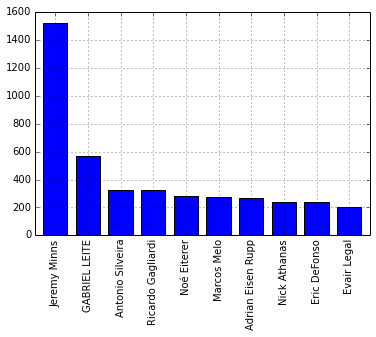
\includegraphics[max size={\textwidth}{\textheight}]{pandas_toGo-slides_files/pandas_toGo-slides_36_1.png}
    \par
    \end{center}
    
            \end{InvisibleVerbatim}
            
        
    
\part{Add new columns}\section{Determine the climate region of the birds}

    % Make sure that atleast 4 lines are below the HR
    \needspace{4\baselineskip}

    
        \vspace{6pt}
        \makebox[0.1\linewidth]{\smaller\hfill\tt\color{nbframe-in-prompt}In\hspace{4pt}{[}48{]}:\hspace{4pt}}\\*
        \vspace{-2.65\baselineskip}
        \begin{ColorVerbatim}
            \vspace{-0.7\baselineskip}
            \begin{Verbatim}[commandchars=\\\{\}]
\PY{n}{tropics} \PY{o}{=} \PY{n}{Image}\PY{p}{(}\PY{l+s}{\PYZsq{}}\PY{l+s}{./images/world.png}\PY{l+s}{\PYZsq{}}\PY{p}{,} \PY{n}{width}\PY{o}{=}\PY{p}{(}\PY{l+m+mi}{300}\PY{p}{,}\PY{l+m+mi}{300}\PY{p}{)}\PY{p}{)}
\PY{c}{\PYZsh{}http://en.wikipedia.org/wiki/Subtropics\PYZsh{}mediaviewer/File:World\PYZus{}map\PYZus{}indicating\PYZus{}tropics\PYZus{}and\PYZus{}subtropics.png}
\end{Verbatim}

            
                \vspace{-0.2\baselineskip}
            
        \end{ColorVerbatim}
    


    % Make sure that atleast 4 lines are below the HR
    \needspace{4\baselineskip}

    
        \vspace{6pt}
        \makebox[0.1\linewidth]{\smaller\hfill\tt\color{nbframe-in-prompt}In\hspace{4pt}{[}49{]}:\hspace{4pt}}\\*
        \vspace{-2.65\baselineskip}
        \begin{ColorVerbatim}
            \vspace{-0.7\baselineskip}
            \begin{Verbatim}[commandchars=\\\{\}]
\PY{n}{tropics}
\end{Verbatim}

            
                \vspace{-0.2\baselineskip}
            
        \end{ColorVerbatim}
    

    

        % If the first block is an image, minipage the image.  Else
        % request a certain amount of space for the input text.
        \needspace{4\baselineskip}
        
        

            % Add document contents.
            
                \makebox[0.1\linewidth]{\smaller\hfill\tt\color{nbframe-out-prompt}Out\hspace{4pt}{[}49{]}:\hspace{4pt}}\\*
                \vspace{-2.55\baselineskip}\begin{InvisibleVerbatim}
                \vspace{-0.5\baselineskip}
    \begin{center}
    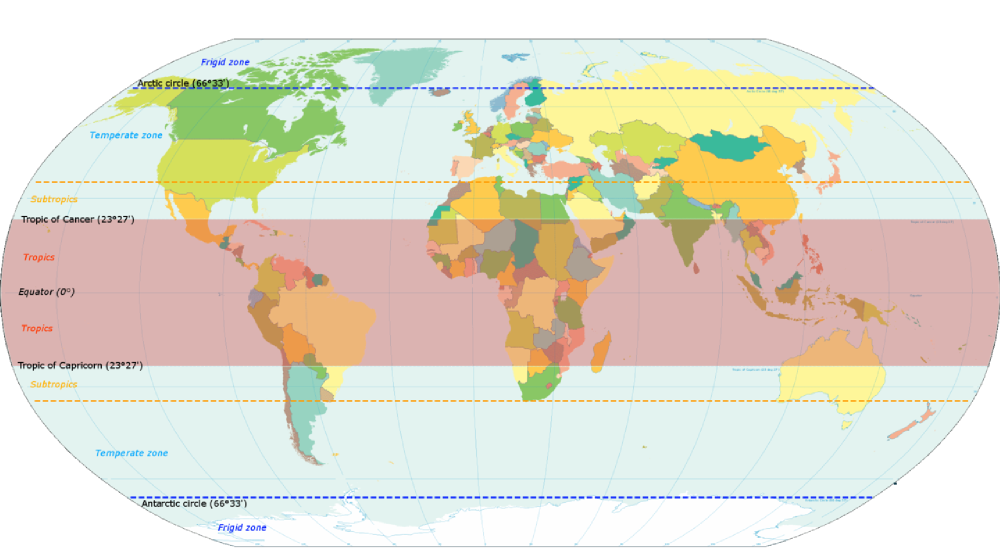
\includegraphics[max size={\textwidth}{\textheight}]{pandas_toGo-slides_files/pandas_toGo-slides_40_0.png}
    \par
    \end{center}
    
            \end{InvisibleVerbatim}
            
        
    
\section{Adding columns}

    % Make sure that atleast 4 lines are below the HR
    \needspace{4\baselineskip}

    
        \vspace{6pt}
        \makebox[0.1\linewidth]{\smaller\hfill\tt\color{nbframe-in-prompt}In\hspace{4pt}{[}36{]}:\hspace{4pt}}\\*
        \vspace{-2.65\baselineskip}
        \begin{ColorVerbatim}
            \vspace{-0.7\baselineskip}
            \begin{Verbatim}[commandchars=\\\{\}]
\PY{n}{tropT} \PY{o}{=} \PY{o}{\PYZhy{}}\PY{l+m+mf}{23.4378} \PY{c}{\PYZsh{} latitude of the tropic of Capricorn}
\PY{c}{\PYZsh{} generate an array with the values of the new column}
\PY{n}{climateRegion} \PY{o}{=} \PY{p}{[}\PY{l+s}{\PYZsq{}}\PY{l+s}{tropical}\PY{l+s}{\PYZsq{}} \PY{k}{if} \PY{n}{item} \PY{o}{\PYZgt{}} \PY{n}{tropT} \PY{k}{else} \PY{l+s}{\PYZsq{}}\PY{l+s}{subtropical}\PY{l+s}{\PYZsq{}} \PY{k}{for} \PY{n}{item} \PY{o+ow}{in} \PY{n}{D}\PY{o}{.}\PY{n}{latitude}\PY{p}{]} \PY{c}{\PYZsh{} using list comprehension}
\PY{c}{\PYZsh{} define que new column}
\PY{n}{D}\PY{p}{[}\PY{l+s}{\PYZsq{}}\PY{l+s}{climate}\PY{l+s}{\PYZsq{}}\PY{p}{]} \PY{o}{=} \PY{n}{climateRegion} 
\PY{n}{D}\PY{o}{.}\PY{n}{head}\PY{p}{(}\PY{p}{)}
\end{Verbatim}

            
                \vspace{-0.2\baselineskip}
            
        \end{ColorVerbatim}
    

    

        % If the first block is an image, minipage the image.  Else
        % request a certain amount of space for the input text.
        \needspace{4\baselineskip}
        
        

            % Add document contents.
            
                \makebox[0.1\linewidth]{\smaller\hfill\tt\color{nbframe-out-prompt}Out\hspace{4pt}{[}36{]}:\hspace{4pt}}\\*
                \vspace{-2.55\baselineskip}\begin{InvisibleVerbatim}
                \vspace{-0.5\baselineskip}
\begin{alltt}      recordist        date   time  \textbackslash{}
0   Daniel Lane  2011-02-24  05:55
1   Daniel Lane  2011-02-24  06:05
2  Eric DeFonso  2011-09-03  18:00
3  Eric DeFonso  2011-09-04  06:00
4  Eric DeFonso  2011-09-04  06:05

                                         location  longitude  latitude
\textbackslash{}
0  10 km S Pocone on Transpantaneira, Mato Grosso   -56.6480  -16.3620
1  10 km S Pocone on Transpantaneira, Mato Grosso   -56.6480  -16.3620
2                    Pantanal Wildlife Center, MT   -56.8764  -16.7581
3                    Pantanal Wildlife Center, MT   -56.8764  -16.7581
4                    Pantanal Wildlife Center, MT   -56.8764  -16.7581

  elevation   climate
0       115  tropical
1       115  tropical
2       110  tropical
3       110  tropical
4       110  tropical

[5 rows x 8 columns]\end{alltt}

            \end{InvisibleVerbatim}
            
        
    


    % Make sure that atleast 4 lines are below the HR
    \needspace{4\baselineskip}

    
        \vspace{6pt}
        \makebox[0.1\linewidth]{\smaller\hfill\tt\color{nbframe-in-prompt}In\hspace{4pt}{[}50{]}:\hspace{4pt}}\\*
        \vspace{-2.65\baselineskip}
        \begin{ColorVerbatim}
            \vspace{-0.7\baselineskip}
            \begin{Verbatim}[commandchars=\\\{\}]
\PY{n}{DsubT} \PY{o}{=} \PY{n}{D}\PY{p}{[}\PY{n}{D}\PY{o}{.}\PY{n}{climate} \PY{o}{==} \PY{l+s}{\PYZsq{}}\PY{l+s}{subtropical}\PY{l+s}{\PYZsq{}}\PY{p}{]}
\PY{n}{DT} \PY{o}{=} \PY{n}{D}\PY{p}{[}\PY{n}{D}\PY{o}{.}\PY{n}{climate} \PY{o}{==} \PY{l+s}{\PYZsq{}}\PY{l+s}{tropical}\PY{l+s}{\PYZsq{}}\PY{p}{]}

\PY{c}{\PYZsh{} plot}
\PY{n}{plt}\PY{o}{.}\PY{n}{scatter}\PY{p}{(} \PY{n}{DT}\PY{o}{.}\PY{n}{longitude}\PY{p}{,} \PY{n}{DT}\PY{o}{.}\PY{n}{latitude}\PY{p}{,} \PY{n}{c} \PY{o}{=} \PY{l+s}{\PYZsq{}}\PY{l+s}{r}\PY{l+s}{\PYZsq{}}\PY{p}{,} \PY{n}{label} \PY{o}{=} \PY{l+s}{\PYZsq{}}\PY{l+s}{tropical}\PY{l+s}{\PYZsq{}}\PY{p}{)}
\PY{n}{plt}\PY{o}{.}\PY{n}{scatter}\PY{p}{(} \PY{n}{DsubT}\PY{o}{.}\PY{n}{longitude}\PY{p}{,} \PY{n}{DsubT}\PY{o}{.}\PY{n}{latitude}\PY{p}{,} \PY{n}{c} \PY{o}{=} \PY{l+s}{\PYZsq{}}\PY{l+s}{g}\PY{l+s}{\PYZsq{}}\PY{p}{,} \PY{n}{label} \PY{o}{=} \PY{l+s}{\PYZsq{}}\PY{l+s}{subtropical}\PY{l+s}{\PYZsq{}}\PY{p}{)}
\PY{n}{plt}\PY{o}{.}\PY{n}{xlabel}\PY{p}{(}\PY{l+s}{\PYZsq{}}\PY{l+s}{longitude}\PY{l+s}{\PYZsq{}}\PY{p}{)}
\PY{n}{plt}\PY{o}{.}\PY{n}{ylabel}\PY{p}{(}\PY{l+s}{\PYZsq{}}\PY{l+s}{latitude}\PY{l+s}{\PYZsq{}}\PY{p}{)}
\PY{n}{plt}\PY{o}{.}\PY{n}{legend}\PY{p}{(}\PY{p}{)}
\PY{n}{plt}\PY{o}{.}\PY{n}{xlim}\PY{p}{(}\PY{o}{\PYZhy{}}\PY{l+m+mi}{90}\PY{p}{,} \PY{o}{\PYZhy{}}\PY{l+m+mi}{10}\PY{p}{)}
\end{Verbatim}

            
                \vspace{-0.2\baselineskip}
            
        \end{ColorVerbatim}
    

    

        % If the first block is an image, minipage the image.  Else
        % request a certain amount of space for the input text.
        \needspace{4\baselineskip}
        
        

            % Add document contents.
            
                \makebox[0.1\linewidth]{\smaller\hfill\tt\color{nbframe-out-prompt}Out\hspace{4pt}{[}50{]}:\hspace{4pt}}\\*
                \vspace{-2.55\baselineskip}\begin{InvisibleVerbatim}
                \vspace{-0.5\baselineskip}
\begin{alltt}(-90, -10)\end{alltt}

            \end{InvisibleVerbatim}
            
                \begin{InvisibleVerbatim}
                \vspace{-0.5\baselineskip}
    \begin{center}
    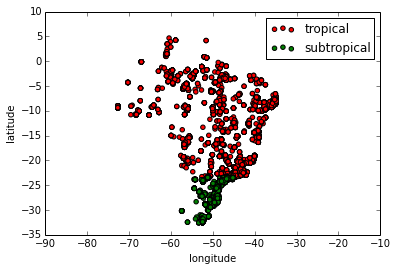
\includegraphics[max size={\textwidth}{\textheight}]{pandas_toGo-slides_files/pandas_toGo-slides_43_1.png}
    \par
    \end{center}
    
            \end{InvisibleVerbatim}
            
        
    
\section{Save as csv}

    % Make sure that atleast 4 lines are below the HR
    \needspace{4\baselineskip}

    
        \vspace{6pt}
        \makebox[0.1\linewidth]{\smaller\hfill\tt\color{nbframe-in-prompt}In\hspace{4pt}{[}38{]}:\hspace{4pt}}\\*
        \vspace{-2.65\baselineskip}
        \begin{ColorVerbatim}
            \vspace{-0.7\baselineskip}
            \begin{Verbatim}[commandchars=\\\{\}]
\PY{n}{D}\PY{o}{.}\PY{n}{to\PYZus{}csv}\PY{p}{(}\PY{l+s}{\PYZsq{}}\PY{l+s}{amazonianBirds\PYZus{}climate.csv}\PY{l+s}{\PYZsq{}}\PY{p}{,} \PY{n}{index} \PY{o}{=} \PY{n+nb+bp}{False}\PY{p}{)}
\end{Verbatim}

            
                \vspace{-0.2\baselineskip}
            
        \end{ColorVerbatim}
    


    % Make sure that atleast 4 lines are below the HR
    \needspace{4\baselineskip}

    
        \vspace{6pt}
        \makebox[0.1\linewidth]{\smaller\hfill\tt\color{nbframe-in-prompt}In\hspace{4pt}{[}39{]}:\hspace{4pt}}\\*
        \vspace{-2.65\baselineskip}
        \begin{ColorVerbatim}
            \vspace{-0.7\baselineskip}
            \begin{Verbatim}[commandchars=\\\{\}]
\PY{c}{\PYZsh{} read what we just saved}
\PY{n}{D\PYZus{}new} \PY{o}{=} \PY{n}{pd}\PY{o}{.}\PY{n}{read\PYZus{}csv}\PY{p}{(}\PY{l+s}{\PYZsq{}}\PY{l+s}{amazonianBirds\PYZus{}climate.csv}\PY{l+s}{\PYZsq{}}\PY{p}{)}
\PY{n}{D\PYZus{}new}\PY{o}{.}\PY{n}{head}\PY{p}{(}\PY{p}{)}
\end{Verbatim}

            
                \vspace{-0.2\baselineskip}
            
        \end{ColorVerbatim}
    

    

        % If the first block is an image, minipage the image.  Else
        % request a certain amount of space for the input text.
        \needspace{4\baselineskip}
        
        

            % Add document contents.
            
                \makebox[0.1\linewidth]{\smaller\hfill\tt\color{nbframe-out-prompt}Out\hspace{4pt}{[}39{]}:\hspace{4pt}}\\*
                \vspace{-2.55\baselineskip}\begin{InvisibleVerbatim}
                \vspace{-0.5\baselineskip}
\begin{alltt}      recordist        date   time  \textbackslash{}
0   Daniel Lane  2011-02-24  05:55
1   Daniel Lane  2011-02-24  06:05
2  Eric DeFonso  2011-09-03  18:00
3  Eric DeFonso  2011-09-04  06:00
4  Eric DeFonso  2011-09-04  06:05

                                         location  longitude  latitude
\textbackslash{}
0  10 km S Pocone on Transpantaneira, Mato Grosso   -56.6480  -16.3620
1  10 km S Pocone on Transpantaneira, Mato Grosso   -56.6480  -16.3620
2                    Pantanal Wildlife Center, MT   -56.8764  -16.7581
3                    Pantanal Wildlife Center, MT   -56.8764  -16.7581
4                    Pantanal Wildlife Center, MT   -56.8764  -16.7581

  elevation   climate
0       115  tropical
1       115  tropical
2       110  tropical
3       110  tropical
4       110  tropical

[5 rows x 8 columns]\end{alltt}

            \end{InvisibleVerbatim}
            
        
    
\section{Group}

    % Make sure that atleast 4 lines are below the HR
    \needspace{4\baselineskip}

    
        \vspace{6pt}
        \makebox[0.1\linewidth]{\smaller\hfill\tt\color{nbframe-in-prompt}In\hspace{4pt}{[}40{]}:\hspace{4pt}}\\*
        \vspace{-2.65\baselineskip}
        \begin{ColorVerbatim}
            \vspace{-0.7\baselineskip}
            \begin{Verbatim}[commandchars=\\\{\}]
\PY{n}{engCounts} \PY{o}{=} \PY{n}{D}\PY{o}{.}\PY{n}{groupby}\PY{p}{(}\PY{l+s}{\PYZsq{}}\PY{l+s}{climate}\PY{l+s}{\PYZsq{}}\PY{p}{)}
\PY{n}{engCounts}\PY{o}{.}\PY{n}{head}\PY{p}{(}\PY{n}{n}\PY{o}{=}\PY{l+m+mi}{3}\PY{p}{)}
\end{Verbatim}

            
                \vspace{-0.2\baselineskip}
            
        \end{ColorVerbatim}
    

    

        % If the first block is an image, minipage the image.  Else
        % request a certain amount of space for the input text.
        \needspace{4\baselineskip}
        
        

            % Add document contents.
            
                \makebox[0.1\linewidth]{\smaller\hfill\tt\color{nbframe-out-prompt}Out\hspace{4pt}{[}40{]}:\hspace{4pt}}\\*
                \vspace{-2.55\baselineskip}\begin{InvisibleVerbatim}
                \vspace{-0.5\baselineskip}
\begin{alltt}                          recordist        date   time  \textbackslash{}
climate
tropical    0           Daniel Lane  2011-02-24  05:55
            1           Daniel Lane  2011-02-24  06:05
            2          Eric DeFonso  2011-09-03  18:00
subtropical 86    Adrian Eisen Rupp  2009-09-30      ?
            87  Bernabe Lopez-Lanus  2007-07-07    ?:?
            88        Frank Lambert  1997-12-17    ?:?

                                                      location
longitude  \textbackslash{}
climate
tropical    0   10 km S Pocone on Transpantaneira, Mato Grosso
-56.648000
            1   10 km S Pocone on Transpantaneira, Mato Grosso
-56.648000
            2                     Pantanal Wildlife Center, MT
-56.876400
subtropical 86       FLONA de Chapecó, Guatambu, Sana Catarina
-52.778000
            87                  SF de Paula, Rio Grande do Sul
-50.583889
            88                    Santa Catarina, near Urubici
-49.580000

                 latitude elevation      climate
climate
tropical    0  -16.362000       115     tropical
            1  -16.362000       115     tropical
            2  -16.758100       110     tropical
subtropical 86 -27.100000       573  subtropical
            87 -29.447778         ?  subtropical
            88 -27.830000      1000  subtropical

[6 rows x 8 columns]\end{alltt}

            \end{InvisibleVerbatim}
            
        
    


    % Make sure that atleast 4 lines are below the HR
    \needspace{4\baselineskip}

    
        \vspace{6pt}
        \makebox[0.1\linewidth]{\smaller\hfill\tt\color{nbframe-in-prompt}In\hspace{4pt}{[}56{]}:\hspace{4pt}}\\*
        \vspace{-2.65\baselineskip}
        \begin{ColorVerbatim}
            \vspace{-0.7\baselineskip}
            \begin{Verbatim}[commandchars=\\\{\}]
\PY{n}{bye}
\end{Verbatim}

            
                \vspace{-0.2\baselineskip}
            
        \end{ColorVerbatim}
    

    

        % If the first block is an image, minipage the image.  Else
        % request a certain amount of space for the input text.
        \needspace{4\baselineskip}
        
        

            % Add document contents.
            
                \makebox[0.1\linewidth]{\smaller\hfill\tt\color{nbframe-out-prompt}Out\hspace{4pt}{[}56{]}:\hspace{4pt}}\\*
                \vspace{-2.55\baselineskip}\begin{InvisibleVerbatim}
                \vspace{-0.5\baselineskip}
    \begin{center}
    
\includegraphics[max size={\textwidth}{\textheight}]{pandas_toGo-slides_files/pandas_toGo-slides_49_0.png}
    \par
    \end{center}
    
            \end{InvisibleVerbatim}
            
        
    


    % Make sure that atleast 4 lines are below the HR
    \needspace{4\baselineskip}

    
        \vspace{6pt}
        \makebox[0.1\linewidth]{\smaller\hfill\tt\color{nbframe-in-prompt}In\hspace{4pt}{[}{]}:\hspace{4pt}}\\*
        \vspace{-2.65\baselineskip}
        \begin{ColorVerbatim}
            \vspace{-0.7\baselineskip}
            \begin{Verbatim}[commandchars=\\\{\}]

\end{Verbatim}

            
                \vspace{0.3\baselineskip}
            
        \end{ColorVerbatim}
    

        

        \renewcommand{\indexname}{Index}
        \printindex

    % End of document
    \end{document}


